\documentclass{article}

\usepackage{fullpage}
\usepackage{color}
\usepackage{amsmath}
\usepackage{url}
\usepackage{verbatim}
\usepackage{graphicx}
\usepackage{parskip}
\usepackage{amssymb}
\usepackage{nicefrac}
\usepackage{listings} % For displaying code
\usepackage{algorithm2e} % pseudo-code

\usepackage{subcaption}
\usepackage[usenames,dvipsnames]{xcolor}

\newcommand{\vect}[1]{\boldsymbol{#1}}
\newcommand\R{\mathbb R}
\newcommand\K{\vect{K}}

%%
%% Julia definition (c) 2014 Jubobs
%%
\lstdefinelanguage{Julia}%
{morekeywords={abstract,break,case,catch,const,continue,do,else,elseif,%
		end,export,false,for,function,immutable,import,importall,if,in,%
		macro,module,otherwise,quote,return,switch,true,try,type,typealias,%
		using,while,begin},%
	sensitive=true,%
	alsoother={\#},%
	morecomment=[l]\#,%
	morecomment=[n]{\#=}{=\#},%
	morestring=[s]{"}{"},%
	morestring=[m]{'}{'},%
}[keywords,comments,strings]%

\lstset{%
	language         = Julia,
	basicstyle       = \ttfamily,
	keywordstyle     = \color{blue},
	stringstyle      = \color{magenta},
	commentstyle     = \color{ForestGreen},
	showstringspaces = false,
}

% Answers
\def\ans#1{\par\gre{Answer: #1}}
%\def\ans#1{} % Comment this line to produce document with answers

% Colors
\definecolor{blu}{rgb}{0,0,1}
\def\blu#1{{\color{blu}#1}}
\definecolor{gre}{rgb}{0,.5,0}
\def\gre#1{{\color{gre}#1}}
\definecolor{red}{rgb}{1,0,0}
\def\red#1{{\color{red}#1}}
\def\norm#1{\|#1\|}

% Math
\def\R{\mathbb{R}}
\def\argmax{\mathop{\rm arg\,max}}
\def\argmin{\mathop{\rm arg\,min}}
\newcommand{\mat}[1]{\begin{bmatrix}#1\end{bmatrix}}
\newcommand{\alignStar}[1]{\begin{align*}#1\end{align*}}
\def\half{\frac 1 2}
\def\cond{\; | \;}

% LaTeX
\newcommand{\fig}[2]{\includegraphics[width=#1\textwidth]{a2f/#2}}
\newcommand{\centerfig}[2]{\begin{center}\includegraphics[width=#1\textwidth]{a2f/#2}\end{center}}
\def\items#1{\begin{itemize}#1\end{itemize}}
\def\enum#1{\begin{enumerate}#1\end{enumerate}}


\begin{document}
	\title{Understanding secondary structure effects on DNA hybridization by visualization tools in large CTMCs \vspace{-0.7em}}
	\author{Chenwei Zhang}
	\date{}
	\maketitle
	\vspace{-3em}



\section{Introduction and related work}

Nucleic acids, including deoxyribonucleic acid (DNA) and ribonucleic acid (RNA) play important roles in the continuity of life. DNA exists in almost every organism and carries genetic information and instructions on protein synthesis. RNA molecules involving three major types such as transfer RNA (tRNA), messenger RNA (mRNA), and ribosomal RNA (rRNA) are mainly functionalized to convert information stored in DNA into proteins. In the past few decades, DNA and RNA nanotechnologies have emerged and been thriving as their abilities to customize molecular self-assembly. Thermodynamics of nucleic acids has been extensively studied. On the other hand, it still leaves many blind spots to understand kinetics due to its sophisticated intrinsic characteristics. Therefore, it is imperative to seek out efficient ways to comprehend and address the mechanism of nucleic acid reaction kinetics. 


Comprehensively understanding DNA hybridization process is important for DNA- and RNA-based biosensor technology. However, few works have been done to analyze the influence of hairpins formation on reaction rates and pathways in DNA hybridization. An illustration in Figure \ref{fig:duplex} shows an example of this reaction process. Although there is an existing work using \textit{oxDNA} which is a coarse-grained model simulating nucleic acid nanotechnology \cite{oxDNA} to simulate hairpin structures in the duplex formation and study their effects on forward and backward reaction rates \cite{schreck}, it is still not very clear what happening and how hairpins contributing during entire transitions of the helix association and dissociation from initial to final states. Here, I propose a more straightforward way to reveal this process by implementing visualization tools to help domain experts to appreciate mechanisms behind the kinetics and help them to design deliberate molecular structures upon DNA nanotechnology. \textit{RiboSketch}, a drawing program to image DNA and RNA secondary structures, can be regarded as a good reference in this project \cite{ribosketch}.

Continuous-time Markov Chains (CTMCs) are commonly utilized to simulate nucleic acid kinetics, such as \textit{Kinfold} \cite{Kinfold}, \textit{Kfold} \cite{Kfold}, and \textit{Multistrand} \cite{Schaeffer} owing to their capabilities to infer equilibrium and non-equilibrium dynamics. A CTMC model of a reaction consists of a state space that includes all possible secondary structures, transitions each of which refers to an elementary step (a single base pair forming or breaking), and transition probabilities that are determined by latent kinetic parameters. A CTMC with reasonable space size can offer direct computation of its dynamics with matrix equation. Whereas one big challenge in real-data CTMCs is that the CTMCs of interest normally have a prohibitively large state space size therefore, it is infeasible to enumerate all the states to compute measures over paths. As a result, appropriate sampling approaches have to be applied to simulate statistically correct trajectories, i.e. sequences of observed states (secondary structures, indicating the hydrogen bonding state of the bases) along with the holding time for each transition \cite{Schaeffer}.

The naivest sampling method is known as Gillespie sampling algorithm \cite{Gillespie} for which trajectories are generated based on the transition rate and holding time of each state. Due to the inefficiency of Gillespie sampling, however, it requires to simulate an extremely large number of samples to acquire reliable estimates. Alternatively, it necessitates other advanced sampling approaches, such as weighted ensemble sampling (WES) \cite{WE_sample}, forward flux sampling (FFS) \cite{FFS1,FFS2}, and kinetic path sampling (KPS) \cite{KPS1,KPS2}. These methods show good performance on CTMCs having relatively small state space sizes and high state occupancies. Instead, for the CTMCs of interest in this study, the state space size is quite large while the occupancy is especially low. It may need to adapt these sampling strategies to realize the purpose.

In this project, I aim to implement a meaningful graphing tool to visualize DNA hybridization kinetics, particularly helix association and dissociation processes and further to understand the effects on hairpins forming and breaking on the course of DNA double-helical strands hybridization and melting. To achieve this goal, I propose a 3D visualization tool with a time slider to display the secondary structure transformation from initial to final states, accompanying by hairpin structure forming and breaking. I am planning to implement Python and Julia to deal with datasets and make plots. And I am also resorting to the software package \textit{DISCOTRESS} \cite{Discotress1,Discotress2} to accomplish the various sampling methods, such as Gillespie, WES, FFS, and KPS. 


\begin{figure}[h]
	\centering
	\vspace*{0.3cm}
	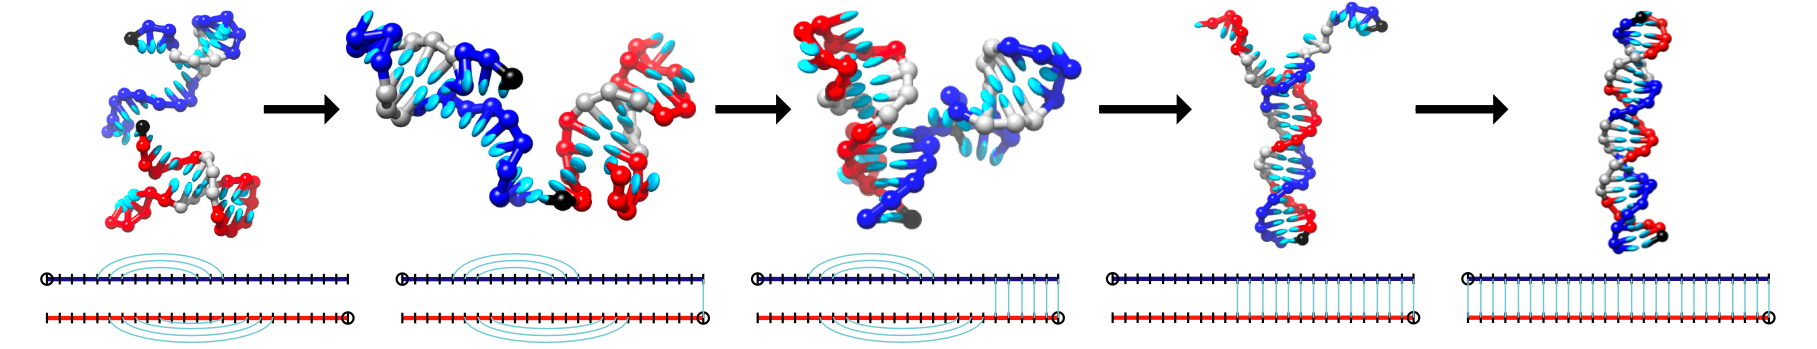
\includegraphics[height=3cm]{latexplots/duplexformation.png}\hspace*{1cm}
	\caption{A typical helix association pathway. Schematic illustrations below the figure indicate hairpin and duplex base pairs present \cite{schreck}.}
	\vspace*{-.3cm}
	\label{fig:duplex}
\end{figure}


\section{Background on CTMCs}
A CTMC is defined as a tuple $C = (S, \K, \pi_0, F)$, where $S$ refers to the set of states, $\K : S\times S \to \R_{\ge 0}$ refers to the rate matrix subject to $\K(s,s) = 0$ for any $s\in S$,  $\pi_0 : S\to [0,1]$ refers to the initial state distribution subject to $\sum_{s\in S} \pi_0(s) = 1$, and $F \subset S$ refers to the set of target (absorbing) states. We define $I \subset S$ as the set of initial states, that is $I = \{ s\in S \, | \, \pi_0(s) > 0\}$. A transition from states $s$ to $s'$ is possible only if $\K(s,s') > 0$. The exit rate matrix, $\vect{E} : S \times S \to \R_{\ge 0}$, is a diagonal matrix defined as $\vect{E} = \sum_{s'\in S} \K(s,s')$ in which each entry represents an exit rate. And the holding time of a state $s$ is exponentially distributed with respect to its corresponding exit rate $\vect{E}(s,s)$. We also define the generating matrix, $\vect{Q} : S\times S \to \R$, as $\vect{Q} = \K-\vect{E}$.

A trajectory is denoted by $(s_0,t_0)$, $(s_1,t_1)$, ..., $(s_n,t_n)$ with n transitions over a CTMC model, where states $s_i$ and holding time $t_i$ subject to $\K(s_i,s_{i+1}) > 0$ and $t_i \in \R_{\geq 0}$ for $i \geq 0$. A path is defined as $s_0$, $s_1$, ..., $s_n$ with n transitions over a CTMC model, where states $s_i$ subject to $\K(s_i,s_{i+1}) > 0$. 


\section{Datasets}
\begin{enumerate}
	\item Modified CTMCs from toy-DNA dataset \cite{DNA23}.
	\item Generating CTMCs from the existing dataset \cite{schreck}.
	\item Synthetic CTMCs.
	\item If applicable, CTMCs from \textit{Multistrand}.
\end{enumerate}


\section{Contributions}

In this project, I am planning to :
\begin{enumerate}
	\item Augment CTMCs from existing experimental data to allow the hairpin forming in the process of helix association and dissociation. And generate CTMCs from the existing dataset \cite{schreck}.
	\item Implement different sampling methods, including Gillespie sampling, WES, FFS, and KPS to obtain statistically correct states and trajectories in large CTMCs.   
	\item Find a meaningful way to index each state and design efficient visualization tools to understand the effect of hairpin on DNA hybridization.
	\item If possible, get insights from Deep Graph Embeddings paper and then find common ground to combine my project with this approach \cite{deepgraph}.
	\item If time permits, implement the pathway elaboration algorithm \cite{PE} and combine it with visualization tools to analyze the relationship between truncated states and hairpin secondary structures in helix association and dissociation.
\end{enumerate}

\clearpage
\bibliographystyle{unsrt}
{\bibliography{references.bib}}


\end{document}